\documentclass[11pt,a4paper]{book}
\usepackage[utf8]{inputenc}
\usepackage[T1]{fontenc}
\usepackage[spanish]{babel}
\usepackage{amsmath}
\usepackage{amsfonts}
\usepackage{amssymb}
\usepackage{graphicx}
\author{Ángel Perea Arias}
\newcommand{\mychapter}[2]{
	\setcounter{chapter}{#1}
	\setcounter{section}{0}
	\chapter*{#2}
	\addcontentsline{toc}{chapter}{#2}
}
\begin{document}
	\title{¡¡¡¡¡ Título temporal !!!!!}
	\date{24 de Mayo del 2020}
	\maketitle
	
	
	\tableofcontents
	%\listoftables
	\listoffigures
	\glossary{GLOSARIO?}
	
	\mychapter{0}{ÍNDICE DE CONTENIDOS}
	\mychapter{0}{ÍNDICE DE FIGURAS}
	\mychapter{0}{ÍNDICE DE TABLAS}
	\mychapter{0}{GLOSARIO}
	\chapter{INTRODUCCIÓN}
		\section{Resumen}
		\section{Motivación}
		El objetivo principal es dotar a la Web Kibotics.org de sondas de almacenamiento de datos y herramientas de visualización para el análisis de estos, ya sean de visitantes a la web, registros de usuarios o uso de los ejercicios.\\
		
		Ofreciendo así a la web y sus administradores de capacidades para recoger, estudiar y valorar los datos aportados para tener una mejor visión global de que rumbo tomar, como está funcionando el servicio, como mejorarlo. \\
		
		Estos datos son imprescindibles para cualquier decisión importante que se deba tomar para mejorar la satisfacción de los usuarios, aumentar la retención, mejorar los contenidos y su distribucion etc... (INCOMPLETO)
	\chapter{OBJETIVOS}
	\chapter{INFRAESTRUCTURA UTILIZADA}
		En este capítulo se describen las diferentes tecnoloías web, de bases de datos y de visualización que se han utilizado en el transcurso del proyecto.
		\section{Tecnologías Web}
			\subsection{Python}
				Python es un lenguaje de programación interpretado, orientado a objetos y de alto nivel. Diseñado para un desarrollo de aplicaciones rapido, se utiliza como lenguaje de scripting y conexión entre otros componentes de un sistema.\\
				
				
				Python es simple, con una sintaxis facil de aprender centrada en la legibilidad del código, consiguiendo así reducir el coste del desarrollo, mantenimiento y ampliación de proyectos.\\
				
				
				Tiene una gran biblioteca de módulos que puede ser facilmente extendida por módulos personalizados escritos en C/Python. Haciendo uso del intalador de paquetes PIP, es posible la instalación e integración de paqueteria en proyectos de manera muy sencilla, así como el cambio de versiones de las mismas.\\
				
				El proyecto comenzó a desarrollarse en Python 2.6 y ha terminado en la versión Python 3.6.9.
				
				
			\subsection{Django}
				Django es un framework Web de alto nivel diseñado para desarrollar aplicaciones en Python, al igual que este, su filosofia se centra en desarrollos rápidos, limpios y en un diseño pragmático.
				Sigue el patrón Model-View-Template (MVT), donde:\\
				
				\begin{itemize}
					\item Model, esta capa del patrón tiene toda la información relativa a las bases de datos: como se almacenan, como se relacionan entre ellas, como validarlas... Manejado por la capa de bases de datos de Django. Toda esta información de configuración se desarrolla y almacena en el fichero Models.py.\\
					
					
					\item View, parte lógica del Framework, se puede ver como una unión entre la capa de modelo y de templates o plantillas. Formado por dos ficheros: urls.py, encargado de llamar a la vista adecuada dependiendo de la URL a la que se acceda y views.py con todas esas vistas que devolverán una respuesta HTTP y en las cuales se consultará la capa Model si fuese necesario.\\
					
					
					\item Template, sección que se encargará del qué y cómo mostrar los datos. Manejado por vistas y plantillas de Django que servirán de bases para la parte Frontend de la Web. Guardado en documentos HTML enriquecidos junto a variables de plantillas Django (\{\{ nombre\_de\_variable \}\}), las cuales permite el uso de, por ejemplo, bucles, operaciones condicionales, diccionarios, insercion de bloques... para generar webs complejas, altamente enriquecidas y dinámicas en muy pocas lineas de código.
					
				\end{itemize}
			
				\begin{figure}
				 	\centering
				 	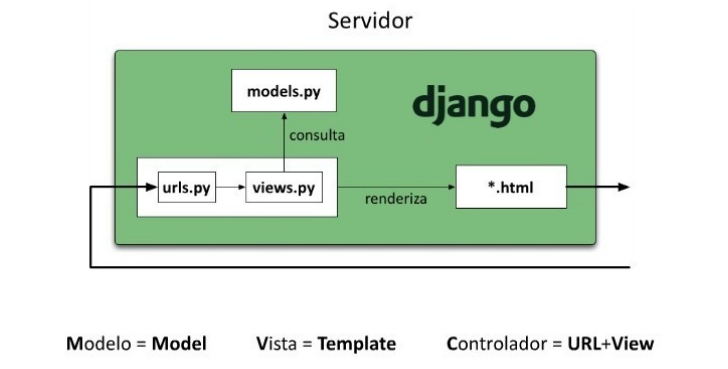
\includegraphics[width=10cm, keepaspectratio]{img/django_MTV.png}
				 	\caption{Patrón MVT Django.}
				 	\label{fig:MTV_Django}
				 \end{figure}
			 
				El proyecto comenzó a desarrollarse en Django 1.9 y ha terminado en la versión Django 1.11.
				
			\subsection{HTML}
				HTML (Hipertextual Markup Lenguaje), es un lenguaje de marcado. Actualmente utilizado para la definición de la estructura básica de los contenidos de una página Web como videos, figuras, iframes... \\
				
				Publicado inicialmente en 1991, su historia se remonta a 1980, cuando Tim Berners-Lee propuso un nuevo sistema para compartir documentos. Actualmente se ha impuesto como el estandar, definido por el World Wide Web Consortium (W3C), el cual ha ido evolucionando versión a versión adoptando todas las nuevas exigencias que ofrecen las Webs actuales en el campo de los recusos multimedia y de interactividad. Actualmente la última versión oficial es HTML 5, la cual proporciona soporte nativo de audio y video, inclusión de la etiqueta canvas, entre otras mejoras.\\
				
				HTML se desarrolla por etiquetas o tags, dentro de las cuales se pueden incluir cada uno de los elementos que conforman una página Web. Dispone de cierta capacidad de aportar estilo y lógica pero estas generalmente se delegan en CSS y JavaScript.
			\subsection{CSS}
				CSS (Cascade Style Sheet), es un lenguaje de reglas en cascada utilizado para dotar de diseño a elementos. El cual define, como se mencionó anteriormente, la estética de un documento HTML y por lo tanto de una página Web. Permite crear webs atractivas y responsivas, esto es, que se adapten al dispositivo en que están siendo vistas, ya sean, por ejemplo, tablets, ordenadores o moviles.\\
				
				Permite mover todas las reglas de estilo
				( tamaños de fuente o imágenes, colores, responsividad de elementos a ciertas resoluciones...) a documentos *.css, evitando así redundancia en documentos *.html, mejorando así la modularidad e independencia dentro de un proyecto.
			\subsection{JavaScript}
				JavaScript es un lenguaje de programación ligero, interpretado, orientado a objetos y dinámico. Utilizado principalmente como lenguaje de scripting para paginas Web, en este campo su papel principal se centra en el desarrollo de lógica en la parte del cliente: acceso al Document Object Model(DOM) de la web, modificación de etiquetas HTML, generación de gráficos en Canvas o gestión de cookies.
				Permite crear nuevo contenido dinámico, asi como controlar archivos multimedia y gracias al uso de API's (Aplication Programming Interface), proporciona a JavaScript de más funcionalidades.
				
				\begin{figure}
					\centering
					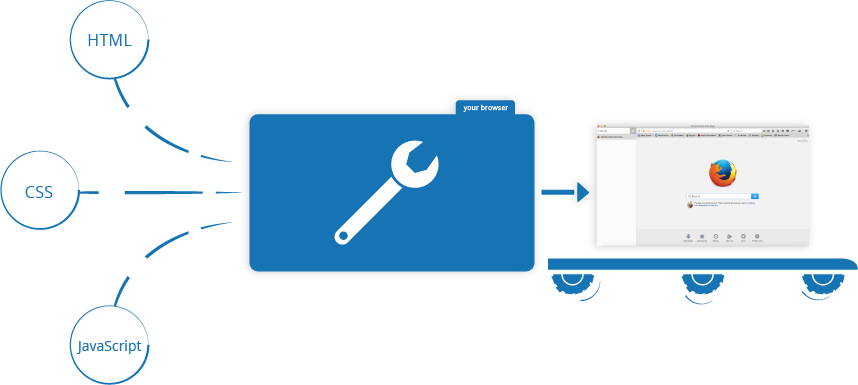
\includegraphics[width=10cm, keepaspectratio]{img/html_css_js.png}
					\caption{Tecnologías web.}
					\label{fig:HTML_CSS_JS}
				\end{figure}
				
				
		\section{Bases de datos}
			\subsection{SQLite}
				SQLite es una libreria ligera, rapida y fiable desarrollada en C. Siendo actualmente el motor de bases de datos SQL más usado en el mundo, utilizado en gran parte de los dispositivos móviles y ordenadores, además de venir de serie en muchas aplicaciones, por ejemplo, Django.\\
				
				
				No necesita de de un servidor para funcionar, hecho por el cual su integracion y despliegue es sencillo, basado en lectura y escritura en un fichero *.sqlite para almacenar toda la información de una base de datos, este fichero es multiplataforma pudiendo así ser migrado entre distintos sistemas de manera muy sencilla. Con un tamaño máximo de 140 terabytes.
				
			\subsection{MongoDB}
				MongoDB es una base de datos NoSQL distribuida, documental (almacenando la información en ficheros BSON, muy similares a JSON), de código abierto y diseñada para ofrecer un nivel productivo alto.\\
				
				Debido a esta estructura, la velocidad en las consultas es muy alta, convirtiendose así en una base de datos ideal para trabajar con grandes cantidades de información que vayan a ser consultados muy frecuentemente.\\
				
				La escalabilidad de MongoDB es muy sencilla, puesto que se ejecuta en clusters, podrá escalar horizontalmente contratando más máquinas, aumentando así la capacidad de procesamiento. Es una base de datos muy utilizada en la industria.
			\subsection{ElasticSearch}
				Elasticsearch es una base de datos. Junto a LogStash y kibana, los tres proyectos open source, forman el Stack ELK. Mediante una simple API Rest realiza consulta, borrado y actualización de documentos. Haciendo uso de objetos JSON tanto para las consultas como para las respuestas de estas, lo que la hace muy facil de usar e integrar en sistemas productivos ya existentes.\\
				
				Basada en Lucene(API para recuperación de información), gracias a esto, permite almacenar información como datos de geolocalización asi como realizar busquedas de texto y autocompletado es muy sencillo.\\
		
				Organizado en nodos, permitirá aumentar la potencia a medida que la demanda de recursos crezca.\\
				
				Datas sus capacidades de amacenar información preparada en índices previamente creados, la consulta de documentos es muy agil puesto que evitamos busquedas en indices no deseados, gracias a esto, se ha convertido en uno de los buscadores de texto más importantes, utilizado por gigantes de internet como Facebook, Netflix o Github.

			\begin{figure}
				\centering
				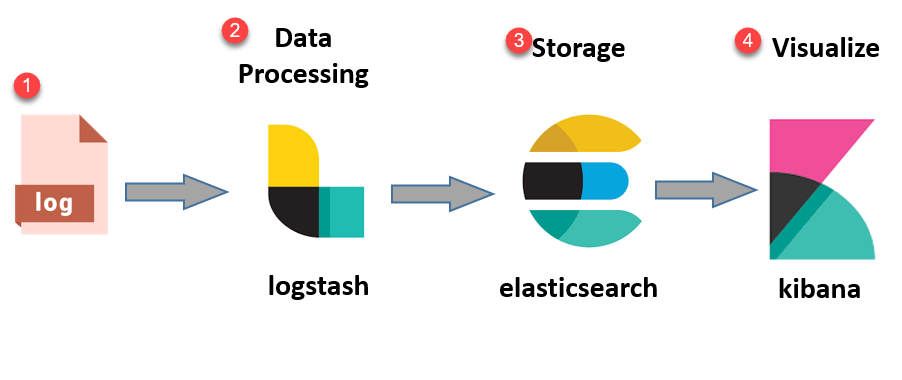
\includegraphics[width=10cm, keepaspectratio]{img/ELK_Stack.png}
				\caption{Stack ELK.}
				\label{fig:MTV_Django}
			\end{figure}
		
		\section{Tecnologías de visualización}
			\subsection{Matplotlib}
				Matplotlib es una libreria de Python que se encarga de la generación de visualizaciones tanto estáticas como animadas. \\
				Proporciona gran variedad de gráficas como mapas de calor, gráficas de barras, histogramas... recordando a Matlab. Ofrece cierta capacidad de estilo y puede ser utilizada junto a otras librerias, para generar gráficos aún más complejos y enriquecidos como mapas geográficos en los que se representarán datos mediante datos de latitud y longitud. \\
				Estas visualizaciones o gráficos podrán ser mostrados en una nueva ventana si utilizamos la libreria en un script o ser renderizadas y devueltas como imágen PNG para su posterior muestra en el servicio Web haciendo uso de la etiqueta HTML <img></img>
			\subsection{Kibana}
				Como se comentó anteriormente, el Stack ELK está compuesto por Kibana como motor de busqueda, procesador de datos y generador de visualizaciones entre otras muchas funcionalidades.\\
				Gracias a su aplicación frontend, la creación de gráficas se simplifica mucho sin ser necesaria la codificación de estas. \\
				Mediante configuración, filtrado y selección de los datos indexados en ElasticSearch se pueden crear múltiples tipos de visualizaciones interactivas (gráficos de barras, gráficos circulares, tablas, histogramas y mapas), y posteriormente ser agrupadas en tableros o Dashboards, los cuales permiten la visualización y posterior filtrado de grandes cantidades de información de forma simultanea y sencilla.\\
				Permite el procesado de los documentos ya indexados en ElasticSearch para crear nuevos campos dinámicos que podrán ser utilizados y representados posteriormente en visualizaciones y estadísticas.
	\chapter{INTEGRACIÓN DE MONGODB \& MATHPLOTLIB EN KIBOTICS WEBSERVER}
		\section{Estado inicial de Kibotics Webserver}
			\subsection{Arquitectura}
			\subsection{Tecnologías}
			\subsection{Logs}
		\section{Desarrollo local}
			\subsection{MongoDB en Kibotics Webserver}
			\subsection{Matplotlib en Kibotics Webserver}
	\chapter{INTEGRACIÓN DEL ELK STACK EN KIBOTICS WEBSERVER}
		\section{Desarrollo local}
			\subsection{ElasticSearch en Kibotics Webserver}
			\subsection{Kibana en Kibotics Webserver}
		\section{Despliegue en producción}
		\section{Generación de recusos de prueba para el desarrollo local}
			\subsection{Receta de instalación de ElasticSearch}
			\subsection{Creación de bases de datos Dummy para Elasticsearch}
			\subsection{Receta de instalación de Kibana}
			\subsection{Creación de bases de datos Dummy para Kibana}
	\chapter{IMPLEMENTACIÓN DE MEJORAS PARA HERRAMIENAS DE GESTIÓN}
		\section{Asignación de permisos individuales}
	\chapter{RESULTADOS}
		\section{Analíticas para visitantes}
		\section{Analíticas para usuarios}
	\chapter{CONCLUSIONES}
		\section{Conclusiones finales}
		\section{Competencias adquiridas}
		\section{Competencias empleadas}
		\section{Trabajos futuros}
	\chapter{REFERENCIAS}
	Django
https://www.djangoproject.com/
	Django MVC
https://uniwebsidad.com/libros/django-1-0/capitulo-5/el-patron-de-diseno-mtv

	HTML 
	https://uniwebsidad.com/libros/xhtml/capitulo-1/breve-historia-de-html
	https://www.w3schools.in/html-tutorial/history/
	
	SQLite
	https://www.sqlite.org/about.html
	
	Elasticsearch
	http://www.arquitectoit.com/elasticsearch/que-es-elasticsearch/
	https://www.ionos.es/digitalguide/servidores/configuracion/que-es-elasticsearch/
	
	Matplotlib
	https://matplotlib.org/
	
	kibana
	https://www.elastic.co/es/what-is/kibana

\end{document}